% !TeX program = xelatex
\documentclass[lang=cn,newtx,a4paper,bibtex]{elegantpaper}

\usepackage{array}
\graphicspath{{figures/}}
\usepackage{tabularx}
\usepackage{makecell}
\usepackage{float}
\usepackage[ruled,linesnumbered]{algorithm2e}
\usepackage{tikz}

\renewcommand{\algorithmcfname}{算法}
\SetKwInput{KwIn}{输入}
\SetKwInput{KwOut}{输出}
\SetKwInput{KwWhere}{where}

\usetikzlibrary{arrows.meta,positioning,fit,shapes.geometric,calc}
\title{%
  函数级代码生成的预算分档编排：统一协议、机制证据与成本前沿\\[4pt]
  \large Budget-Tiered Test-Time Orchestration for Function-Level Code Generation%
}
\author{薛沁晨}
\date{}

\begin{document}

\maketitle

% Abstract
\begin{abstract}
在 API 计费与上下文长度约束下，函数级代码生成的部署效果取决于测试时计算如何组织，而非单次生成本身。本文将问题表述为可复现的\textbf{预算分档编排协议}：在单一实现与统一统计口径下，把从单步到级联的行为固定为四个可对照档位，使不同预算形态可在同一执行器与同一评测口径下比较。

主实验在 HumanEval 与 MBPP 两条函数级基准上联合报告通过率、调用次数与总 token，并给出经验收益率 $\rho$ 刻画各档边际与累计成本--收益关系。结果表明：在更难、更杂的任务分布上，分档编排带来更宽的通过率提升空间；在易饱和分布上，增益更多体现为残差段收束与成本重分配。机制上，静态结构难度分更适合作为\textbf{预算分配先验}而非运行失败分类器；multiset 随机路由对照用于分离 hard 覆盖率与结构对齐的贡献；反馈回注形态对照表明，压缩回注在精度几乎不变的前提下可显著降低 token 开销。

部署上，中预算侧重结构化主链与失败回注修补，高预算侧重候选扩展并在可选 refine 上做精度与 token 的折中。
\keywords{函数级代码生成；测试时计算；预算分档；失败修补；级联编排}
\end{abstract}

\begingroup
\renewcommand{\abstractname}{Abstract}
\renewcommand{\abstracttextfont}{\small\normalfont\noindent\ignorespaces}
\begin{abstract}
Under API pricing and context-length constraints, the deployment effectiveness of function-level code generation depends on how test-time computation is organized, rather than on a single generation attempt alone. This paper formulates the problem as a reproducible \textbf{budget-tiered orchestration protocol}: under one implementation and one unified accounting interface, behaviors from single-step generation to cascaded workflows are fixed into four comparable tiers, so that different budget forms can be compared under the same executor and evaluation protocol.

The main experiments jointly report pass rate, number of calls, and total tokens on the HumanEval and MBPP function-level benchmarks, and introduce an empirical gain rate $\rho$ to characterize both marginal and cumulative cost--benefit relationships across tiers. Results show that tiered orchestration provides broader room for pass-rate improvement on harder and more heterogeneous task distributions; on easier and more saturated distributions, the gains are more reflected in residual-set convergence and cost reallocation. Mechanistically, static structural difficulty scores are more suitable as \textbf{budget-allocation priors} than as runtime failure classifiers; the multiset random-routing control separates the contribution of hard-slot coverage from structural alignment; and the feedback-injection comparison shows that compressed feedback can substantially reduce token cost while keeping accuracy nearly unchanged.

For deployment, the medium-budget setting emphasizes a structured main chain and failure-feedback repair, whereas the high-budget setting emphasizes candidate expansion and trades off accuracy against token cost through optional refine steps.

\par\vskip2ex\noindent\normalfont{\bfseries Keywords: } function-level code generation; test-time computation; budget tiering; failure repair; cascade orchestration
\end{abstract}
\endgroup


% Switch to two-column layout for the body
\twocolumn

% Body sections
\section{引言}
\label{sec:introduction}

大语言模型已经成为函数级代码生成系统的核心组件。HumanEval 与 MBPP 等基准表明，强模型能够在相当比例的短函数任务上通过单次生成得到可运行实现\cite{chen2021evaluating,austin2021program}。真实部署进一步关心接口计费、上下文长度与调用预算共同约束下的系统编排。对同一失败样本，重新采样、执行反馈修补、结构化重链、候选扩展与执行筛选都会改变通过率和成本之间的关系\cite{li2022alphacode,chen2024selfdebug,shinn2023reflexion,gou2024critic,li2025sstar}。

现有研究已经分别验证了若干有效组件：执行反馈能够修补错误程序，候选扩展与筛选能够提高通过率，反思或批判式提示能够改善复杂任务。然而这些组件在工程系统中往往以多个开关叠加出现，若执行器、统计口径或默认提示模板不同，最终收益很难归因到预算组织本身。本文关注的正是这一层问题：在同一实现中逐级解锁不同测试时计算投向，同时记录通过率、调用次数与令牌成本。

本文将这一口径称为\textbf{预算分档编排}。协议把函数级代码生成流程组织为四个语义明确的档位：单步档作为最低成本基线；单步+修补档在失败后引入执行反馈；分流+重链与救援档依据结构难度先验选择重路径，并将失败信息压缩回注；级联档在高预算下扩展候选集并用执行结果筛选。四档共享同一外层闭环，差异只在新增预算投向，使成本--收益关系能够被直接比较。

该协议同时给出机制层面的解释路径。结构难度分承担预算排序作用，用于把更复杂的样本优先送入重路径；固定轻/重路径多重集的随机对照用于隔离覆盖率和结构对齐；压缩回注与完整回溯的对照刻画反馈形式对修补收益和令牌成本的影响；级联消融进一步区分候选扩展和后处理精修的贡献。这样，端到端结果和模块机制可以在同一实验口径下相互印证。

本文的主要贡献如下：

1）\textbf{协议贡献}：提出面向函数级代码生成的预算分档编排协议，在统一执行器、统一判定与统一记账下比较单步、修补、分流救援与级联四类预算形态，将测试时计算从调用次数多少转化为预算投向差异。

2）\textbf{机制贡献}：围绕分流、反馈与级联三个环节给出机制实验。结构难度分被建模为预算分配先验，固定轻/重路径多重集对照检验结构对齐效果，压缩反馈与完整回溯的五随机种子对照评估回注形式。

3）\textbf{评测贡献}：在 HumanEval 与 MBPP 双基准上报告四档三随机种子主结果，并同时给出通过率、平均调用次数、总令牌与经验收益率 $\rho$。实验显示，MBPP 上分档收益更充分，HumanEval 上主要体现为高位残差收束，二者共同展示了预算编排在不同任务分布下的价值。

全文组织如下。第~\ref{sec:related} 节梳理代码生成评测、执行反馈修补与测试时扩展相关工作；第~\ref{sec:formulation} 节给出问题定义、预算档位和成本记账口径；第~\ref{sec:method} 节描述分流、救援与级联的实现机制；第~\ref{sec:experiments} 节报告主结果与消融；第~\ref{sec:discussion} 节讨论部署含义、机制边界与局限；第~\ref{sec:conclusion} 节总结全文。

\section{相关工作}
\label{sec:related}

\subsection{函数级代码生成评测}

函数级代码生成通常以题面、函数签名和单元测试评测模型能否生成可执行程序。HumanEval\cite{chen2021evaluating} 与 MBPP\cite{austin2021program} 是该方向最常用的基准，前者规模较小、题面相对集中，后者覆盖更广的 Python 任务。随后，APPS\cite{hendrycks2021apps} 与 CodeXGLUE\cite{lu2021codexglue} 扩展了竞赛题和多任务代码评测范围，DS-1000\cite{lai2023ds1000} 与 EvalPlus\cite{liu2023evalplus} 分别强化了数据科学代码和测试充分性评测，LiveCodeBench\cite{jain2024livecodebench} 进一步强调时间切分和污染控制。

上述基准的共同价值在于提供可执行判定，使代码生成研究能够超越文本相似度指标。本文沿用 HumanEval 与 MBPP，是因为二者均为函数级任务，适合在同一执行器下比较测试时编排策略。除通过率外，本文同步记录调用次数与令牌成本，以反映接口部署中的实际约束。

\subsection{执行反馈驱动的程序修补}

执行反馈为代码生成提供了自然的外部验证信号。Self-Debug\cite{chen2024selfdebug} 与 Reflexion\cite{shinn2023reflexion} 表明，模型可以利用执行错误或语言化反馈修补失败程序。CRITIC\cite{gou2024critic} 与 Self-Refine\cite{madaan2023selfrefine} 进一步展示了外部工具反馈或自反馈在迭代修正中的作用。AgentCoder\cite{huang2024agentcoder} 与 CodeT\cite{chen2023codet} 则从多智能体协作或生成测试的角度利用执行信号筛选候选实现。CodeRL\cite{le2022coderl} 说明单元测试结果也可以作为训练阶段的强化学习信号；近期自调试研究中的 LLM-guided self-debugging\cite{adnan2025llmsguided} 与 Revisit Self-Debugging\cite{chen2025revisit} 继续讨论自生成测试与调试反馈在代码生成中的有效边界。这一路线的核心问题在于反馈如何进入下一轮生成。完整回溯包含较多运行环境文本，会增加令牌成本；压缩反馈则把错误类型、关键片段和修补方向组织成更短的约束。

本文继承执行反馈修补的基本思想，并将其放入预算分档协议中考察：反馈修补是中预算档位的主要计算投向。本文单独比较压缩反馈与完整回溯，在相同流程下观察通过率与令牌成本的差异。

\subsection{测试时计算扩展与候选筛选}

另一条相关路线是通过测试时计算扩展提高覆盖率。AlphaCode\cite{li2022alphacode} 展示了大规模候选生成与筛选在竞赛级代码生成中的作用，后续 S*\cite{li2025sstar} 进一步讨论候选数量、筛选策略与成本之间的关系。面向成本控制，Hybrid LLM\cite{ding2024hybrid} 使用路由器在大小模型之间分配查询，LLM Cascades\cite{yue2024cascades} 则用级联结构降低强模型调用成本。更一般地，链式思维\cite{wei2022cot} 与自一致性\cite{wang2023selfconsistency} 说明，多条推理轨迹可以提升复杂任务的答案稳定性。ReAct\cite{yao2023react} 与 Toolformer\cite{schick2023toolformer} 从工具交互角度扩展了测试时决策空间，Tree of Thoughts\cite{yao2023tot} 则把显式搜索引入复杂问题求解。这些方法说明，在模型能力既定时，额外候选或额外推理路径可以提高命中可行解的概率，同时带来调用次数和令牌成本的增长。

本文的级联档与该思路一致，即把高预算主要投入候选扩展和执行筛选。通过关闭候选扩展、限制精修次数等消融，本文区分主增益来源与边际后处理，并用经验收益率 $\rho$ 描述追加预算的成本前沿。与强调单一技巧提升的工作不同，本文进一步关注同一实现下的预算组织问题：当分流、修补、候选扩展和精修同时可用时，系统需要以可比较、可复现和可记账的方式组织它们。因此，本文先在固定评测口径下给出端到端结果，再用机制实验解释预算投向的收益来源。

\section{问题定义与协议}
\label{sec:formulation}

本节给出本文研究对象的形式化定义。本文把测试时计算视为可记账的资源分配问题：在同一代码生成任务集合上，给定一个预算档位，系统决定是否继续调用模型、如何使用执行反馈、是否扩展候选集，并在统一执行器下记录收益与成本。

\subsection{函数级代码生成与统一判定}
\label{sec:formal-objective}

设函数级代码生成数据集为
\begin{equation}
    \mathcal{D}=\{x_i\}_{i=1}^{N},
\end{equation}
其中 $x_i$ 包含题面、函数签名以及测试接口。给定预算档位 $b$，编排器生成一个或多个候选程序，最终提交候选 $y_i^{(b)}$ 至执行器 $E$，得到二值判定
\begin{equation}
    z_i^{(b)} = E(y_i^{(b)}) \in \{0,1\}.
\end{equation}
通过率定义为 $p_b=N^{-1}\sum_i z_i^{(b)}$。除通过率外，本文对每题记录模型调用次数 $c_i^{(b)}$ 与令牌消耗 $t_i^{(b)}$，并汇总得到平均调用次数与总令牌。这里的关键约束是：所有档位共享同一执行器、同一超时与同一测试判定口径，差异仅来自预算档位允许的后续动作。

这一设定把问题从某一提示是否更好，转化为某一预算形态能在相同统计口径下带来多少收益。后文主结论以同协议内的四档结果为核心证据，跨模型结果与细粒度消融用于解释机制来源。

图~\ref{fig:budget_accounting_protocol} 概括了本文的记账口径：预算档位只改变编排器允许采取的动作，判定与成本记录保持统一。

\begin{figure}[t]
\centering
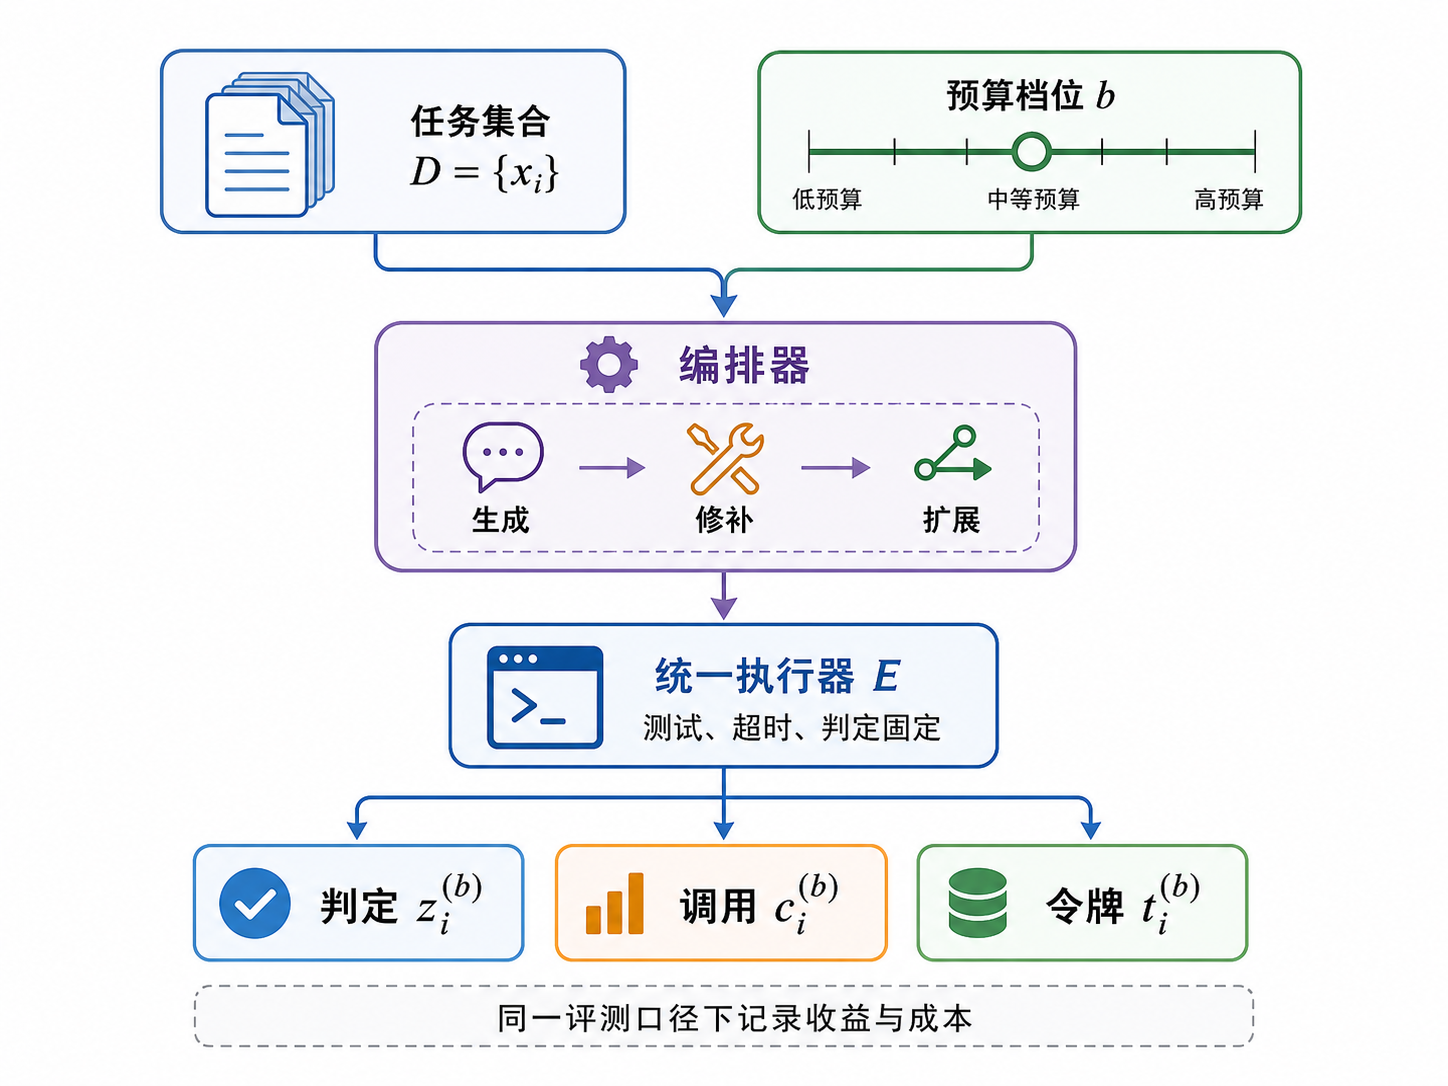
\includegraphics[width=0.98\linewidth]{gpt-fig1-budget-accounting.png}
\caption{统一预算记账协议}
\label{fig:budget_accounting_protocol}
\end{figure}


\subsection{预算档位与语义约束}
\label{sec:tier-protocol}

预算分档协议将测试时编排限制为四个语义清晰的档位。档位越高，解锁的计算投向越丰富：从单次生成，到失败修补，再到难度分流下的重路径，最后到候选扩展与执行筛选。表~\ref{tab:tier_mapping} 给出语义档位与仓库实现模式之间的对应关系。其中第三档在双基准上共用 \texttt{difficulty\_aware\_plus} 实现，命令行预算别名仅作为复现入口，正文仍按语义档位定义；第一档日志别名 \texttt{base\_direct} 与 \texttt{single\_step} 同义。

\begin{table*}[htbp]
\centering
\small
\caption{预算语义档位与实现模式映射}
\label{tab:tier_mapping}
\begin{tabularx}{\textwidth}{p{2.6cm} p{3.5cm} X}
\toprule
语义档位 & 实现模式 & 允许的主要计算投向 \\
\midrule
单步 & \texttt{single\_step} & 单次生成与执行判定；作为最低成本基线 \\
单步+修补 & \texttt{single\_step\_repair} & 在单次失败后使用执行反馈做有限修补 \\
分流+重链与救援 & \texttt{difficulty\_aware\_plus} & 依据结构难度进入轻/重路径，重路径启用结构化主链与失败后救援 \\
级联 & \texttt{workflow\_cascade} & 多候选扩展、执行筛选以及有限精修/融合 \\
\bottomrule
\end{tabularx}
\end{table*}

该映射有两个作用。首先，它统一模式名与预算档位，减少解释歧义；其次，它为成本解释提供统一坐标，使通过率上升和令牌增长能够放在同一成本--收益框架下讨论。

\subsection{成本记账与经验收益率}
\label{sec:accounting}

真实部署中，调用次数只反映部分成本。一次长上下文修补可能比多次短调用更昂贵，级联阶段的候选组织也会推高令牌消耗。因此，本文以总令牌作为主成本代理，以平均调用次数作为辅助指标。若某档 $b$ 相对前一档 $b-1$ 的通过率增量为 $\Delta p=p_b-p_{b-1}$，额外令牌为 $\Delta t=t_b-t_{b-1}$，则定义经验性边际收益率
\begin{equation}
    \rho = \frac{\Delta p}{\Delta t}.
\end{equation}
为便于跨档比较，实验节还报告相对单步档的累计收益率
\begin{equation}
    \rho_b^{(\mathrm{cum})}=
    \frac{p_b-p_{\mathrm{single}}}{t_b-t_{\mathrm{single}}}.
\end{equation}
这两个量用于解释新增令牌带来的通过率收益，帮助判断不同档位的边际效率。

\subsection{证据层级}
\label{sec:evidence-levels}

本文按三层组织证据。第一层是双基准四档三随机种子主结果，用于刻画预算分档的整体前沿。第二层是多模型单随机种子扫描，用于观察不同基础模型下的档位形态。第三层是机制消融，包括阈值扫描、流程开关、反馈形态和随机路由对照，用于回答预算主要花在哪里、收益来自哪个模块。

这一组织方式贯穿全文，使主结果、跨模型形态和机制解释各自承担清晰角色。

\section{预算分档编排方法}
\label{sec:method}

本节描述四档协议在实现层面的组织方式。系统围绕同一个外层闭环运行：读入任务、生成候选、执行测试、记录结果；若失败，则在当前预算档位允许的范围内追加修补、重链、救援或级联。将程序生成与执行反馈连接起来的思想可追溯到执行引导程序综合和 REPL 式程序搜索\cite{chen2019execution,ellis2019write}。整体流程见图~\ref{fig:overall_framework}。

\begin{figure*}[t]
\centering
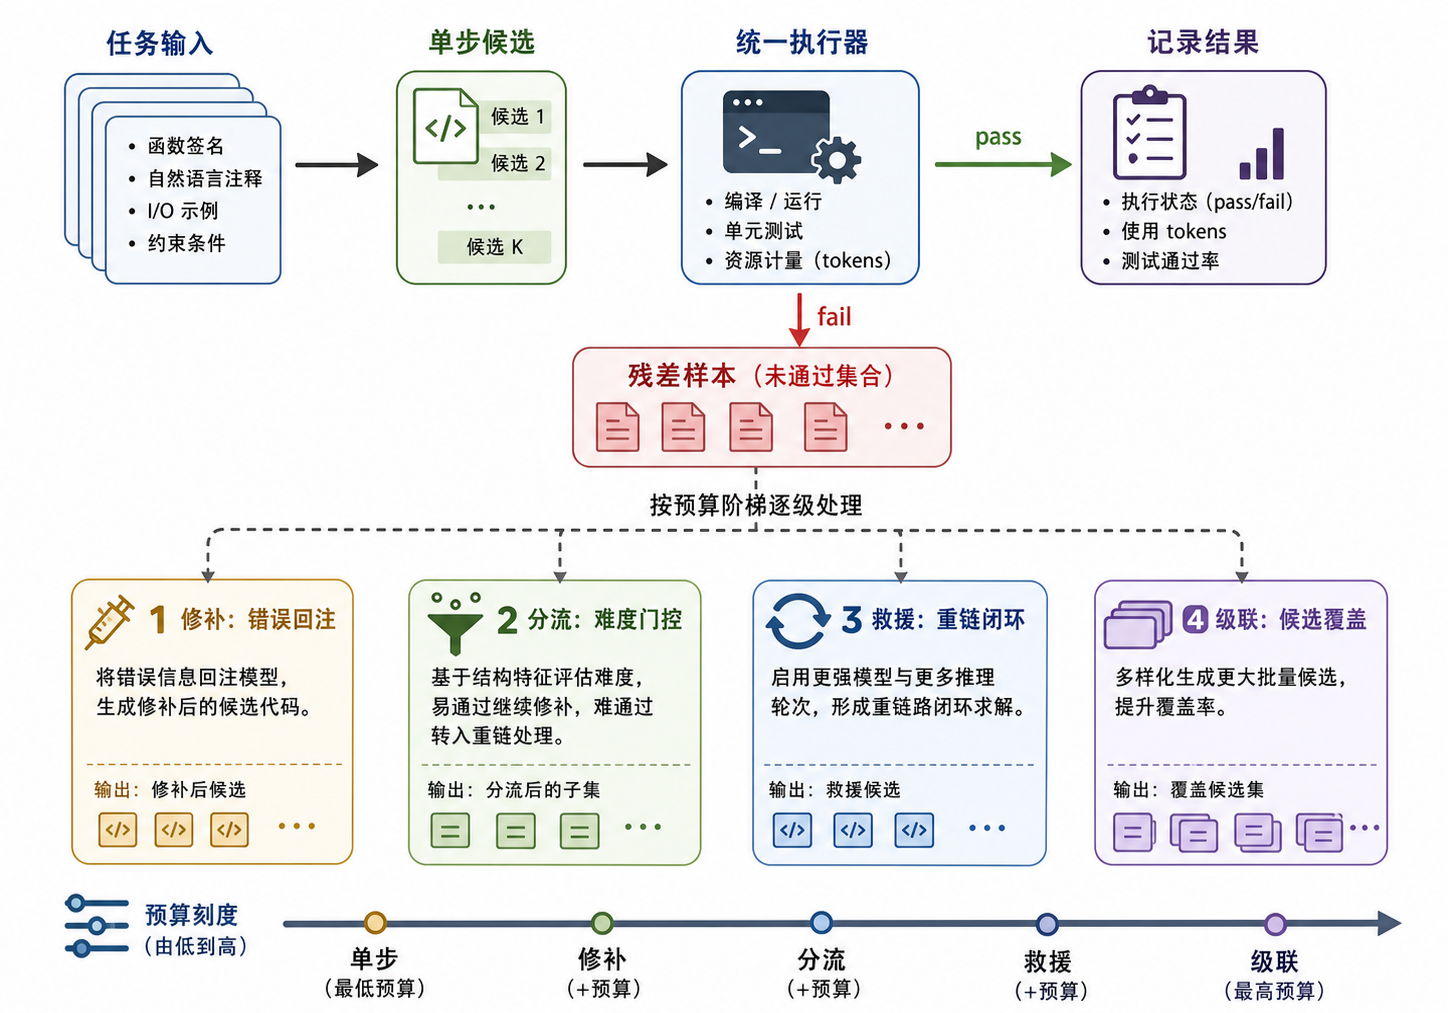
\includegraphics[width=0.98\textwidth]{gpt-fig2-overall-framework.png}
\caption{预算分档编排整体框架}
\label{fig:overall_framework}
\end{figure*}


\subsection{总体流程}
\label{sec:overview-flow}

对每个任务 $x_i$，系统首先生成单步候选并交由执行器判定。候选通过后流程结束；候选失败后，低档位直接结束或进入轻量修补，高档位根据结构难度、执行反馈与候选池状态决定后续动作。这样的组织把新增预算集中在\textbf{单步未能覆盖的残差样本}上。

四档的差异可以概括如下。单步档只做一次生成，是最低成本基线；单步+修补档在失败后追加有限修补调用，检验执行反馈的边际价值；分流+重链与救援档先判断样本是否进入重路径，再使用结构化提示、错误压缩与候选救援处理复杂失败；级联档进一步扩展候选集合，并用执行筛选和可选精修组织高预算搜索。

算法~\ref{alg:budget_tier} 给出单个样本上的预算分档编排逻辑。算法只刻画档位间的控制流，结构难度打分、失败反馈压缩与级联候选扩展的具体实现分别在后续小节展开。

\begin{algorithm*}[t]
\SetAlgoLined
\small
\caption{预算分档编排协议}
\label{alg:budget_tier}
\KwIn{任务 $x_i$，预算档位 $b$，模型 $p_\theta$，执行器 $E$，结构阈值 $\tau_{\mathrm{eff}}$}
\KwOut{最终候选 $y_i$，判定 $z_i$，调用次数 $c_i$，令牌消耗 $t_i$}
\KwWhere{$\textsc{Single}\prec\textsc{Repair}\prec\textsc{Route}\prec\textsc{Cascade}$ defines the budget order}
$y^\star \leftarrow \mathrm{Generate}(p_\theta, x_i)$\;
$(z^\star,e^\star) \leftarrow E(y^\star)$; update $c_i,t_i$\tcp*{single-step baseline}
\If{$z^\star=1$ \textbf{or} $b=\textsc{Single}$}{
    \Return $(y^\star,z^\star,c_i,t_i)$\;
}
\If{$b \succeq \textsc{Repair}$}{
    $\tilde{x}_i \leftarrow \mathrm{Concat}(x_i,\phi(e^\star))$\tcp*{compressed feedback}
    $y \leftarrow \mathrm{Generate}(p_\theta,\tilde{x}_i)$; $(z,e)\leftarrow E(y)$; update $c_i,t_i$\;
    \lIf{$z=1$}{$(y^\star,z^\star,e^\star)\leftarrow(y,z,e)$}
    \If{$z^\star=1$ \textbf{or} $b=\textsc{Repair}$}{
        \Return $(y^\star,z^\star,c_i,t_i)$\;
    }
}
$s_i \leftarrow \mathrm{Difficulty}(x_i)$; $r_i\leftarrow\mathbb{I}(s_i\ge\tau_{\mathrm{eff}})$\;
\If{$r_i=1$}{
    $(y,z,e)\leftarrow\mathrm{HeavyChain}(x_i,e^\star)$; update $c_i,t_i$\;
    \lIf{$z=1$}{$(y^\star,z^\star,e^\star)\leftarrow(y,z,e)$}
}
\If{$z^\star=0$}{
    $(y,z,e)\leftarrow\mathrm{Rescue}(x_i,e^\star)$; update $c_i,t_i$\;
    \lIf{$z=1$}{$(y^\star,z^\star,e^\star)\leftarrow(y,z,e)$}
}
\If{$b=\textsc{Cascade}$ \textbf{and} $z^\star=0$}{
    $\mathcal{Y}\leftarrow\mathrm{ExpandCandidates}(x_i,y^\star,e^\star)$\;
    $(y^\star,z^\star)\leftarrow\mathrm{SelectByExecutor}(\mathcal{Y},E)$; update $c_i,t_i$\;
}
\Return $(y^\star,z^\star,c_i,t_i)$\;
\end{algorithm*}

\subsection{结构难度路由}
\label{sec:routing}

难度路由用于在进入重路径之前完成一次粗粒度预算筛分。它承担\textbf{预算分配先验}的角色：结构上更复杂的题目更可能需要额外上下文、结构化提示或候选扩展，因而优先进入重路径。

图~\ref{fig:routing_decision} 展示了结构分数到轻/重路径的门控关系。

\begin{figure*}[t]
\centering
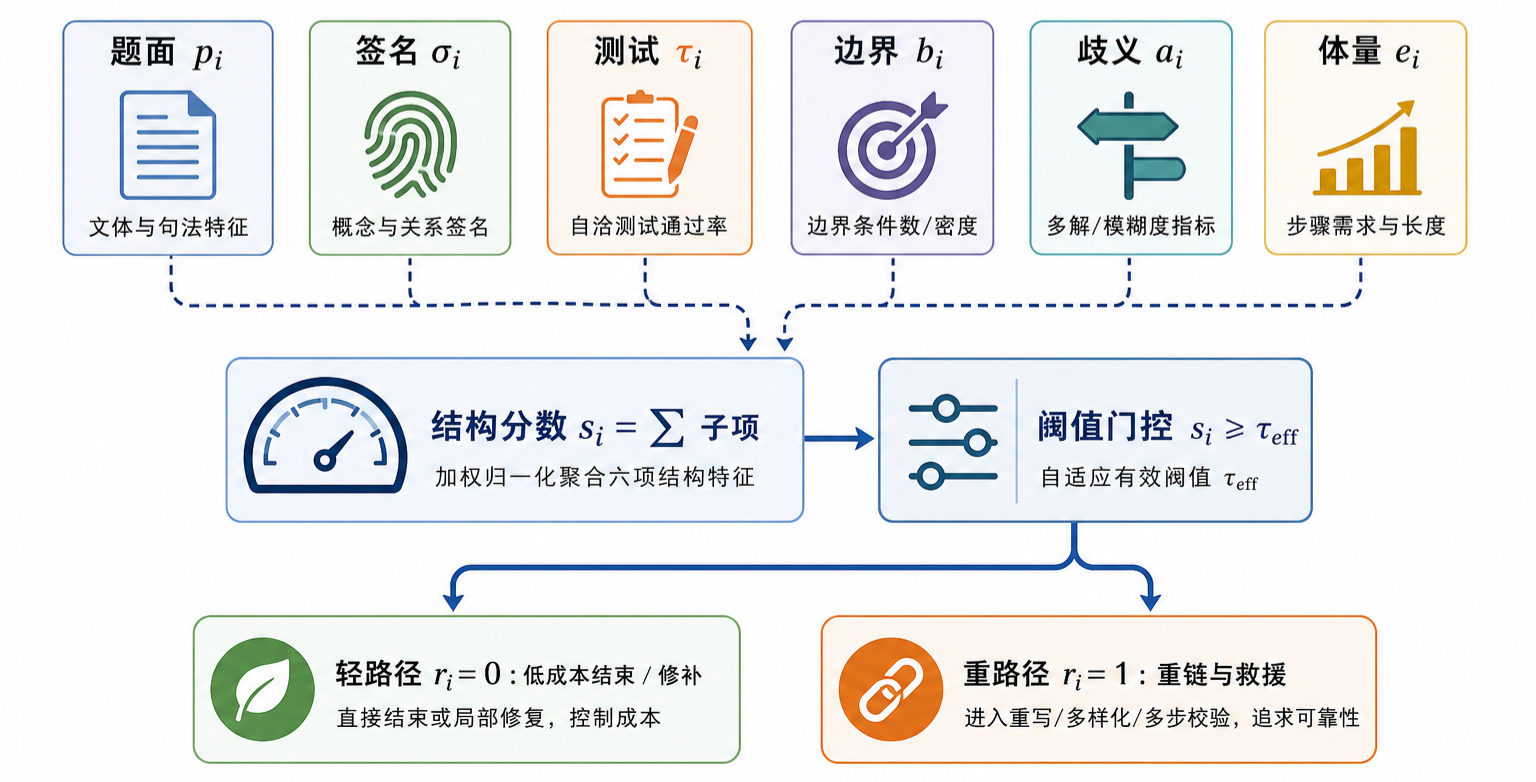
\includegraphics[width=0.98\textwidth]{gpt-fig3-routing-decision.png}
\caption{结构难度路由决策}
\label{fig:routing_decision}
\end{figure*}


记样本 $x_i$ 的结构难度分数为 $s_i$。实现中的 v2 打分器将分数拆为题面复杂度、签名/接口复杂度、测试复杂度、边界条件密度、题面歧义以及有界体量项：
\begin{equation}
\label{eq:difficulty}
s_i = p_i+\sigma_i+\tau_i+b_i+a_i+e_i.
\end{equation}
其中 $p_i,\sigma_i,\tau_i,b_i,a_i$ 分别对应题面、签名、测试、边界与歧义五类子项，$e_i$ 为由题面长度、测试长度、断言数量等构成的有界体量项。各子项由固定启发式规则加权并裁剪上限，总分由题面结构确定。

路由决策写为
\begin{equation}
    r_i=\mathbb{I}(s_i\ge \tau_{\mathrm{eff}}),
\end{equation}
其中 $\tau_{\mathrm{eff}}$ 为配置中的结构阈值，主实验第三档默认使用 $1.6$。$r_i=1$ 表示进入重路径主链，$r_i=0$ 表示停留在轻路径。阈值越低，重路径覆盖率越高，通常带来更高成本和更高通过率上限；阈值越高，成本下降，同时覆盖样本减少。该关系由第~\ref{sec:experiments} 节的阈值消融检验。

为分离重路径覆盖率与结构对齐的影响，仓库实现了 \texttt{random\_permute\_matched} 对照：先按结构分得到本批样本的轻/重路径标签多重集，再固定随机种子置换标签，使重路径数量与默认结构路由完全一致，但题目与重路径槽位的对应被打乱。该对照刻画固定覆盖率下的结构对齐效果。

\subsection{失败反馈与救援链}
\label{sec:rescue}

执行失败后，系统把失败信息转化为下一轮生成可利用的局部约束。其基本思路与 Self-Debug、Reflexion 等执行反馈工作一致\cite{chen2024selfdebug,shinn2023reflexion}，也与利用工具反馈进行自我修正的研究方向相近\cite{gou2024critic,madaan2023selfrefine}。本文进一步考察反馈形式对令牌成本与修补收益的影响。

在分流+重链与救援档中，系统先根据执行器返回的 \texttt{check\_correctness} 字符串判断失败形态。该判断由规则函数完成：未闭合字符串、语法非法等更倾向于替换生成；缺参、参数数量不匹配、名称未定义或缩进错误等归入修补；其余进入更保守的替换或救援路径。当单步与结构化双路径均失败时，系统比较二者错误标签，以决定后续修补轮数。

压缩后的回注包记为
\begin{equation}
\begin{aligned}
\phi(e_i^{(1)})=\operatorname{Concat}\bigl(&
\textit{错误类型},
\textit{截断摘要},\\
&
\textit{规则片段},
\textit{定向修补提示}
\bigr).
\end{aligned}
\end{equation}
其中 $e_i^{(1)}$ 为第一次失败反馈。第二轮上下文可写作
\begin{equation}
\tilde{x}_i^{(2)}=\operatorname{Concat}(x_i,\phi(e_i^{(1)})),
\end{equation}
并据此生成新候选
\begin{equation}
y_i^{(2)} \sim p_{\theta}(\cdot\mid \tilde{x}_i^{(2)}).
\end{equation}
该表达式说明失败信息如何被裁剪并进入下一轮上下文。图~\ref{fig:rescue_loop} 展示了这一闭环。

\begin{figure}[t]
\centering
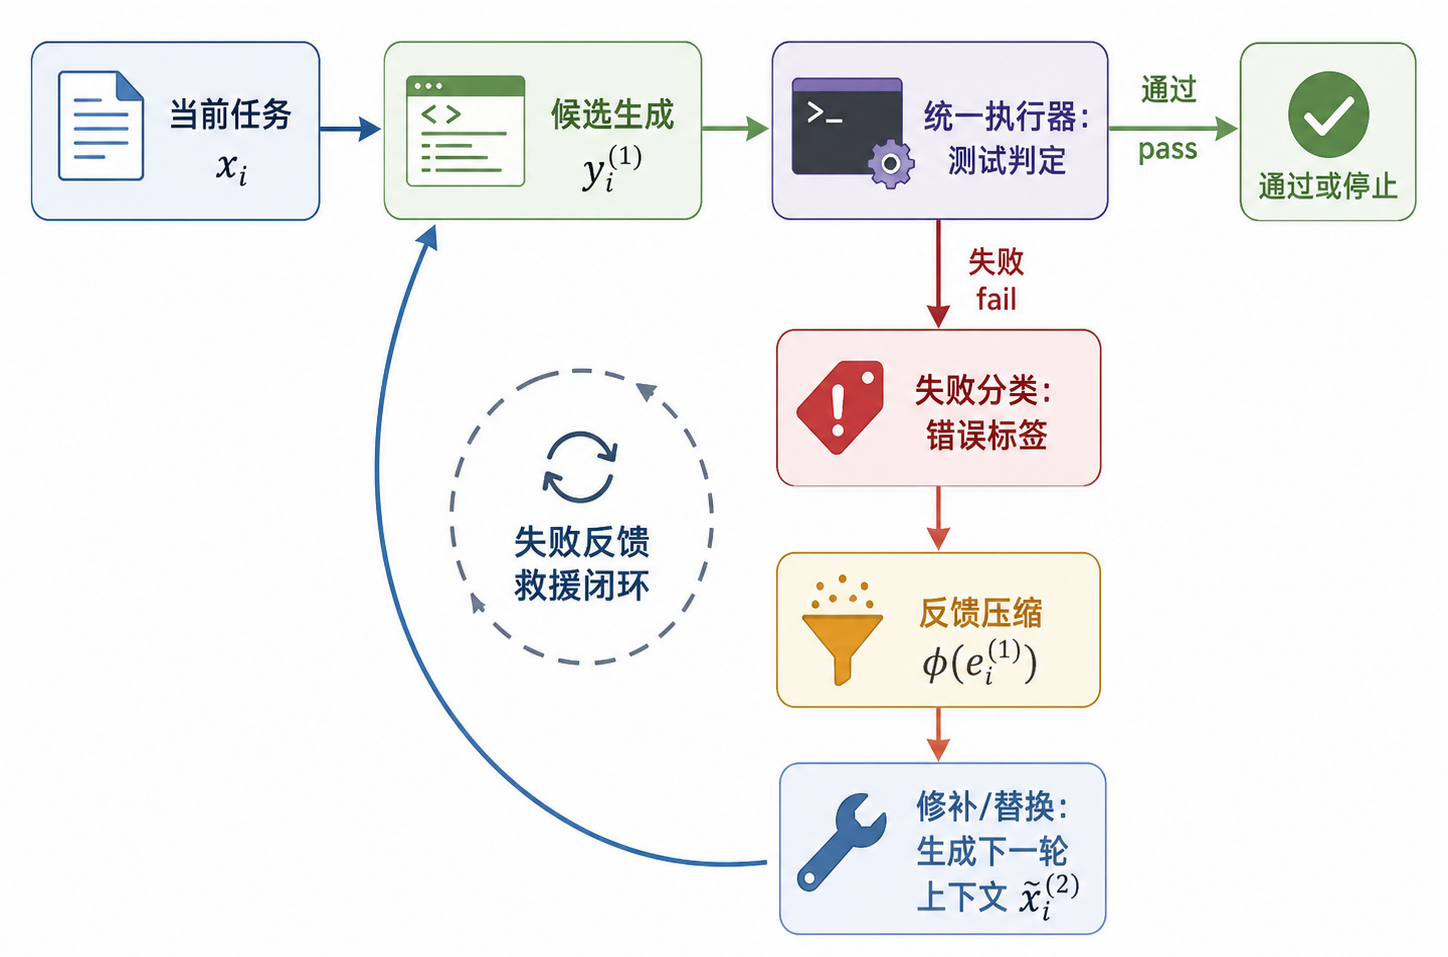
\includegraphics[width=0.98\linewidth]{gpt-fig4-rescue-loop.png}
\caption{失败反馈救援闭环}
\label{fig:rescue_loop}
\end{figure}


本文在实验中比较压缩回注与完整回溯两种形态。五随机种子结果显示，压缩回注保持相近通过率，同时平均令牌更低，因此作为默认回注形式。

\subsection{高预算级联}
\label{sec:cascade}

级联档把新增预算转向候选空间覆盖。其流程包括三层：候选扩展层生成额外候选，执行筛选层用统一测试选择可行实现，后处理层对进入候选池的样本做有限精修或融合。该设计与测试时扩展的基本思想一致，即通过候选扩展提高命中可行解的概率\cite{li2022alphacode,li2025sstar}。

实现上，级联主链按基线候选、额外候选扩展、执行筛选和可选后处理的顺序运行。额外候选阶段的生成次数受全局上限、路由表与执行 top-$k$ 共同约束；实际执行数为生成数与 top-$k$ 的较小值。可行解指在统一执行器下通过官方单元测试的候选实现。若候选扩展已产生可行解，精修只作为精度--成本微调。

第~\ref{sec:experiments} 节的级联消融显示，额外候选扩展是高预算档的主增益来源；精修相关开关更多体现为令牌与少量精度之间的折中。级联档的核心是用候选覆盖换取更高上限。

\subsection{实现不变式与可比性控制}
\label{sec:method-invariants}

为保证不同预算档位之间的比较只反映编排动作差异，本文在实现中固定三类不变式。第一，所有档位共享同一执行器、测试接口、超时设置和通过判定函数，避免把评测口径差异混入预算收益。第二，结构难度分数只由题面、签名和测试结构等预执行信息计算，不使用执行结果或人工标签；随机置换路由对照进一步把重路径覆盖率与结构对齐效果分开。第三，失败回注只使用执行器返回的错误信息及规则化摘要，不引入参考答案或额外人工修正。上述约束使四档协议能够作为同一测试时计算空间中的可记账比较，而不是彼此独立的提示模板集合。

\section{实验}
\label{sec:experiments}

\subsection{评测协议与数据集}
\label{sec:eval-protocol}

本文在 HumanEval 164 题与 MBPP 清洗集 427 题上评测预算分档编排。两者均属于函数级代码生成任务，能够使用同一执行器和同一通过判定口径；差异在于任务分布和动态范围。HumanEval 在当前强模型设定下更接近饱和区间，适合观察残差收束；MBPP 题面更杂、规模更大，更适合观察预算扩展带来的成本--收益曲线。

主结果统一使用 \texttt{claude-sonnet-4-6}，并对四个预算档位报告三随机种子（42、78、132）的均值与样本标准差。多模型结果和多数细粒度消融采用随机种子 42，用于补充观察档位形态和模块机制。

评价指标包括通过率、平均调用次数与总令牌。通过率衡量任务正确性，调用次数反映调度复杂度，总令牌作为接口成本的主代理。表~\ref{tab:protocol_constraints} 汇总本文的公平性约束。

\begin{table*}[htbp]
\centering
\small
\caption{实验协议约束}
\label{tab:protocol_constraints}
\begin{tabularx}{\textwidth}{p{2.8cm} X}
\toprule
约束项 & 本文约束 \\
\midrule
数据口径 & MBPP 清洗集 427 + HumanEval 164 \\
模型与版本 & 主结果统一 \texttt{claude-sonnet-4-6}；多模型结果单独列出 \\
随机性控制 & 主表四档三随机种子统计；E2 反馈形态对照五随机种子；多重集随机路由对照为随机种子 42 单次配对 \\
执行与判定 & 统一执行器、超时、测试调用方式与通过判定口径 \\
比较轴线 & 主结论以同协议内预算分档双基准主结果为准；多模型表和消融表解释形态与机制 \\
成本指标 & 同时报告通过率、平均调用次数、总令牌 \\
\bottomrule
\end{tabularx}
\end{table*}

\subsection{RQ1：预算分档是否形成可解释前沿}
\label{sec:rq1}

表~\ref{tab:main_results} 给出四个预算档位在双基准上的主结果。主结果统一使用 \texttt{claude-sonnet-4-6}，报告三随机种子（42、78、132）的均值与样本标准差。策略列使用第~\ref{sec:tier-protocol} 节的语义档位，括号中只保留实现模式标识，便于复现。表中边际 $\rho$ 相对上一档计算，单位为百分点/万令牌；当相邻两档令牌不增时不定义。

\begin{table*}[htbp]
\centering
\small
\caption{预算分档编排主结果}
\label{tab:main_results}
\begin{tabularx}{\textwidth}{@{}p{2.2cm} >{\raggedright\arraybackslash}X c c c c@{}}
\toprule
数据集 & 策略 & 通过率(\%) & 平均调用次数 & 总令牌 & 边际$\rho$ \\
\midrule
MBPP & 单步（\texttt{single\_step}） & $82.51\pm0.48$ & $1.000\pm0.000$ & $113{,}922\pm5{,}621$ & --- \\
MBPP & 单步+修补（\texttt{single\_step\_repair}） & $86.65\pm0.24$ & $1.177\pm0.001$ & $141{,}207\pm4{,}393$ & 1.52 \\
MBPP & 分流+重链与救援（\texttt{difficulty\_aware\_plus}） & $88.52\pm0.24$ & $1.483\pm0.009$ & $218{,}327\pm2{,}138$ & 0.24 \\
MBPP & 级联（\texttt{workflow\_cascade}） & $91.72\pm0.36$ & $1.639\pm0.021$ & $321{,}177\pm11{,}854$ & 0.31 \\
\midrule
HumanEval & 单步（\texttt{single\_step}） & $97.56\pm0.00$ & $1.000\pm0.000$ & $64{,}938\pm116$ & --- \\
HumanEval & 单步+修补（\texttt{single\_step\_repair}） & $99.19\pm0.35$ & $1.020\pm0.003$ & $66{,}925\pm1{,}588$ & 8.19 \\
HumanEval & 分流+重链与救援（\texttt{difficulty\_aware\_plus}，v2，$\tau$=1.6） & $99.39\pm0.00$ & $1.067\pm0.010$ & $75{,}151\pm1{,}064$ & 0.25 \\
HumanEval & 级联（\texttt{workflow\_cascade}，默认基线） & $99.80\pm0.35$ & $1.055\pm0.010$ & $73{,}847\pm1{,}422$ & --- \\
\bottomrule
\end{tabularx}
\end{table*}

图~\ref{fig:cost_pass_frontier} 将主结果放到统一成本--通过率坐标中，以便观察两个基准在不同动态范围下的前沿形态。

\begin{figure*}[t]
\centering
% Shared color TikZ styles for the paper figures.
\colorlet{paperBlue}{blue!9!white}
\colorlet{paperBlueLine}{blue!55!black}
\colorlet{paperTeal}{teal!10!white}
\colorlet{paperTealLine}{teal!55!black}
\colorlet{paperAmber}{orange!15!white}
\colorlet{paperAmberLine}{orange!60!black}
\colorlet{paperRose}{red!9!white}
\colorlet{paperRoseLine}{red!55!black}
\colorlet{paperViolet}{violet!10!white}
\colorlet{paperVioletLine}{violet!55!black}
\colorlet{paperInk}{black!72}

\tikzset{
  paperfig/.style={
    font=\small,
    >=Stealth,
    line cap=round,
    line join=round
  },
  paperline/.style={
    -{Stealth[length=2.1mm,width=1.6mm]},
    line width=0.58pt,
    draw=paperInk
  },
  paperdash/.style={
    paperline,
    dashed,
    draw=black!48
  },
  paperbox/.style={
    draw=black!58,
    line width=0.58pt,
    rounded corners=2pt,
    fill=white,
    align=center,
    inner xsep=5pt,
    inner ysep=5pt,
    minimum height=8mm
  },
  paperdata/.style={
    paperbox,
    fill=paperBlue,
    draw=paperBlueLine
  },
  paperproc/.style={
    paperbox,
    fill=paperTeal,
    draw=paperTealLine
  },
  papermodel/.style={
    paperbox,
    fill=paperAmber,
    draw=paperAmberLine,
    line width=0.65pt
  },
  paperout/.style={
    paperbox,
    fill=paperRose,
    draw=paperRoseLine,
    line width=0.65pt,
    font=\small\bfseries
  },
  paperstate/.style={
    paperbox,
    fill=paperViolet,
    draw=paperVioletLine
  },
  papernote/.style={
    font=\scriptsize,
    align=center,
    text=black!70,
    fill=white,
    inner sep=1.4pt
  },
  paperaxis/.style={
    line width=0.45pt,
    draw=black!72
  },
  papergrid/.style={
    line width=0.25pt,
    draw=black!15
  },
  paperplot/.style={
    line width=0.95pt,
    draw=paperBlueLine
  },
  paperplotA/.style={
    line width=0.95pt,
    draw=paperBlueLine
  },
  paperplotB/.style={
    line width=0.95pt,
    draw=paperAmberLine
  },
  papermark/.style={
    circle,
    draw=paperBlueLine,
    fill=white,
    line width=0.55pt,
    inner sep=1.6pt
  },
  papermarkA/.style={
    papermark,
    draw=paperBlueLine,
    fill=paperBlue
  },
  papermarkB/.style={
    papermark,
    draw=paperAmberLine,
    fill=paperAmber
  }
}

\resizebox{0.95\textwidth}{!}{%
\begin{tikzpicture}[paperfig, x=1mm, y=1mm]
  \begin{scope}
    \node[font=\small\bfseries] at (27,43) {MBPP};
    \draw[paperaxis] (0,0) -- (55,0);
    \draw[paperaxis] (0,0) -- (0,36);
    \foreach \x/\lab in {0/10,18/18,36/26,54/34} {
      \draw[papergrid] (\x,0) -- (\x,36);
      \node[font=\scriptsize, below] at (\x,0) {\lab};
    }
    \foreach \y/\lab in {0/80,12/84,24/88,36/92} {
      \draw[papergrid] (0,\y) -- (55,\y);
      \node[font=\scriptsize, left] at (0,\y) {\lab};
    }
    \draw[paperplotA] (3.1,6.5) -- (9.3,17.1) -- (26.6,21.9) -- (49.8,30.1);
    \foreach \x/\y/\lab in {3.1/6.5/单步,9.3/17.1/修补,26.6/21.9/分流,49.8/30.1/级联} {
      \node[papermarkA] at (\x,\y) {};
      \node[font=\scriptsize, above] at (\x,\y) {\lab};
    }
    \node[font=\scriptsize] at (27,-7) {总令牌（万）};
    \node[font=\scriptsize, rotate=90] at (-8,18) {通过率（\%）};
  \end{scope}

  \begin{scope}[xshift=76mm]
    \node[font=\small\bfseries] at (27,43) {HumanEval};
    \draw[paperaxis] (0,0) -- (55,0);
    \draw[paperaxis] (0,0) -- (0,36);
    \foreach \x/\lab in {0/6.2,18/6.8,36/7.4,54/8.0} {
      \draw[papergrid] (\x,0) -- (\x,36);
      \node[font=\scriptsize, below] at (\x,0) {\lab};
    }
    \foreach \y/\lab in {0/97,12/98,24/99,36/100} {
      \draw[papergrid] (0,\y) -- (55,\y);
      \node[font=\scriptsize, left] at (0,\y) {\lab};
    }
    \draw[paperplotB] (8.8,6.7) -- (14.8,26.3) -- (39.5,28.7) -- (35.5,33.6);
    \foreach \x/\y/\lab in {8.8/6.7/单步,14.8/26.3/修补,39.5/28.7/分流,35.5/33.6/级联} {
      \node[papermarkB] at (\x,\y) {};
      \node[font=\scriptsize, above] at (\x,\y) {\lab};
    }
    \node[font=\scriptsize] at (27,-7) {总令牌（万）};
    \node[font=\scriptsize, rotate=90] at (-8,18) {通过率（\%）};
  \end{scope}
\end{tikzpicture}%
}
\caption{预算分档的成本--通过率前沿}
\label{fig:cost_pass_frontier}
\end{figure*}


MBPP 上四档呈现清晰的预算扩展轨迹：通过率从 $82.51\%$ 提升到 $91.72\%$，总令牌从约 $1.14\times 10^5$ 增至约 $3.21\times 10^5$。单步+修补的边际 $\rho$ 最高，说明执行反馈修补是最具性价比的第一层增益；分流救援与级联继续提高上限，并对应更高令牌成本。HumanEval 上，单步已经达到 $97.56\%$，后续增益集中在少量残差样本。两组结果共同说明，预算分档的收益与任务分布动态范围密切相关。

\subsection{RQ2：分档形态是否跨模型保持一致}
\label{sec:rq2}

表~\ref{tab:model_results_mbpp} 与表~\ref{tab:model_results_he} 报告多个基础模型在四档协议下的通过率，用于观察分档形态的可迁移性。两表均采用随机种子 42 单次运行，数值单位为通过率百分比。

\begin{table*}[htbp]
\centering
\caption{MBPP 多模型预算分档结果}
\label{tab:model_results_mbpp}
\begin{tabular}{lcccc}
\toprule
模型 & 单步 & 单步+修补 & 分流+重链与救援 & 级联 \\
\midrule
claude-sonnet-4-6 & 82.51 & 86.65 & 88.52 & 91.72 \\
gpt-5.4 & 72.13 & 77.75 & 79.39 & 85.48 \\
gpt-5.3-codex & 71.90 & 78.92 & 79.39 & 83.84 \\
qwen3-coder-plus & 71.90 & 76.58 & 79.63 & 81.97 \\
qwen3-30b-a3b-instruct-2507 & 68.38 & 75.18 & 77.99 & 80.80 \\
gemini-3.1-flash-lite-preview & 73.54 & 76.81 & 79.39 & 80.09 \\
qwen-plus & 70.73 & 75.18 & 77.28 & 79.63 \\
\bottomrule
\end{tabular}
\end{table*}

\begin{table*}[htbp]
\centering
\caption{HumanEval 多模型预算分档结果}
\label{tab:model_results_he}
\begin{tabular}{lcccc}
\toprule
模型 & 单步 & 单步+修补 & 分流+重链与救援 & 级联 \\
\midrule
claude-sonnet-4-6 & 97.56 & 99.19 & 99.39 & 99.80 \\
gemini-3.1-flash-lite-preview & 97.56 & \textbf{98.78} & \textbf{99.39} & 98.78 \\
gpt-5.3-codex & 95.12 & 97.56 & 98.78 & 99.39 \\
gpt-5.4 & 95.12 & 97.56 & 97.56 & 98.78 \\
qwen3-coder-plus & 95.73 & 97.56 & 98.78 & 98.17 \\
qwen3-30b-a3b-instruct-2507 & 92.68 & 95.73 & 97.56 & 96.34 \\
qwen-plus & 92.68 & 97.50 & 96.34 & 95.12 \\
\bottomrule
\end{tabular}
\end{table*}

在 MBPP 上，多数模型呈现逐档抬升，说明协议对不同基础模型具有相似的粗形态。HumanEval 上整体接近饱和，部分模型在高档出现回落或持平，表明高预算级联更适合承担上限探索，而中预算修补和分流档更适合常规部署。

\subsection{RQ3：关键机制如何影响前沿}
\label{sec:mechverify}

本节分析三类机制：结构路由、反馈回注和模块开关。除特别说明外，细粒度消融多在 MBPP 上以随机种子 42 单次运行；MBPP 的动态范围更宽，更适合承载模块排序和成本前沿分析。

\subsubsection{结构分的预算先验作用}

本文先检验静态结构分与运行失败之间的关系。在任务级样本上使用逻辑回归 5 折交叉验证时，首轮失败与需重路由两类标签的 ROC-AUC 分别约为 0.471 与 0.473；加入扩展静态特征后，AUC 约升至 0.51。结果表明，结构分的价值主要体现在预算排序：它把结构更复杂的题目优先送入重路径，再由端到端前沿、阈值扫描和路由对照共同体现收益。

\subsubsection{固定多重集随机路由对照}

表~\ref{tab:route_random_multiset} 报告 \texttt{difficulty\_aware\_plus} 档在 $b{=}0.6$、$\tau{=}1.6$ 下的配对结果，模型为 \texttt{claude-sonnet-4-6}，采用随机种子 42 单次运行。结构路由为默认设置；随机对照为第~\ref{sec:routing} 节定义的固定多重集随机置换。两者在同一数据集上的轻/重路径数量完全一致，因此比较的是同一重路径覆盖率下，题目与槽位对齐方式的影响。

\begin{table*}[htbp]
\centering
\small
\caption{固定多重集随机路由对照}
\label{tab:route_random_multiset}
\begin{tabularx}{\textwidth}{@{}p{2.4cm} >{\raggedright\arraybackslash}p{3.6cm} >{\raggedright\arraybackslash}p{3.6cm} c c@{}}
\toprule
数据集 & 结构路由（通过/总） & 随机对照（通过/总） & 结构路由总令牌 & 随机对照总令牌 \\
\midrule
MBPP 427 & 383/427（89.70\%） & 379/427（88.76\%） & 267{,}878 & 234{,}912 \\
HumanEval 164 & 163/164（99.39\%） & 163/164（99.39\%） & 77{,}683 & 76{,}563 \\
\bottomrule
\end{tabularx}
\end{table*}

在本次配对中，MBPP 上结构路由多通过 4 题，平均调用次数为 677 次，高于随机对照的 640 次；HumanEval 上通过数相同，平均调用次数分别为 178 次和 177 次，令牌差异也较小。结果显示，在固定重路径覆盖率下，结构对齐能在更复杂分布上带来额外收益，并形成相应成本。

\subsubsection{反馈回注形态}

表~\ref{tab:e2_feedback_format_5seed} 比较压缩反馈与完整回溯。该实验在 MBPP 427 上使用 \texttt{difficulty\_aware\_plus} 档与 $b=0.6$，报告五随机种子的均值与样本标准差；除修补阶段回注形态外，其余模型、预算、任务与路由配置保持一致。

\begin{table*}[htbp]
\centering
\caption{E2 反馈形态对照}
\label{tab:e2_feedback_format_5seed}
\begin{tabularx}{\textwidth}{p{3.2cm} c c c X}
\toprule
回注形态 & 通过数 & pass@1(\%) & 总令牌 & 解读 \\
\midrule
压缩回注 & $379.4\pm3.85$ & $88.852\pm0.900$ & $229{,}713\pm7{,}558$ & 均值令牌更低；通过率保持相近 \\
完整回溯 & $379.0\pm1.41$ & $88.756\pm0.334$ & $233{,}180\pm2{,}781$ & 均值令牌更高；保留完整错误上下文 \\
\bottomrule
\end{tabularx}
\end{table*}

两组通过率均值差约 $0.096$ 个百分点，低于各自标准差量级；令牌均值差约 $3{,}467$。压缩回注以更短上下文取得相近通过率，适合作为默认回注形态。

\subsubsection{阈值、主链与级联开关}

表~\ref{tab:ablation_06_threshold} 在 MBPP 427 上使用 v2 打分器和随机种子 42 单次运行，扫描结构阈值 $\tau$。较低阈值提高重路径覆盖率和令牌成本，较高阈值降低成本并减少重路径样本。

\begin{table*}[htbp]
\centering
\caption{分流+重链与救援档阈值消融}
\label{tab:ablation_06_threshold}
\begin{tabularx}{\textwidth}{p{2.0cm} p{2.2cm} c c c X}
\toprule
阈值 $\tau$ & 轻/重路径 & pass@1 & 平均调用 & 总令牌 & 解读 \\
\midrule
$\tau$=1.0 & 92 / 335 & \textbf{382/427} & 1.646 & 255,523 & 精度最高，但成本明显更高 \\
$\tau$=1.1 & 127 / 300 & 381/427 & 1.597 & 243,529 & 轻微降分，成本下降 \\
$\tau$=1.4 & 187 / 240 & 380/427 & 1.511 & 220,825 & 进入更平衡区间 \\
$\tau$=1.6 & 213 / 214 & 381/427 & 1.489 & 217,510 & 默认点，精度/成本折中 \\
$\tau$=1.7 & 224 / 203 & 379/427 & 1.476 & 217,534 & 再提高阈值出现降分 \\
$\tau$=1.8 & 254 / 173 & 376/427 & \textbf{1.447} & \textbf{205,909} & 成本最低，但精度损失明显 \\
\bottomrule
\end{tabularx}
\end{table*}

图~\ref{fig:threshold_tradeoff} 展示同一扫描中的精度--成本位置，默认阈值位于较平衡的区间。

\begin{figure}[t]
\centering
% Shared color TikZ styles for the paper figures.
\colorlet{paperBlue}{blue!9!white}
\colorlet{paperBlueLine}{blue!55!black}
\colorlet{paperTeal}{teal!10!white}
\colorlet{paperTealLine}{teal!55!black}
\colorlet{paperAmber}{orange!15!white}
\colorlet{paperAmberLine}{orange!60!black}
\colorlet{paperRose}{red!9!white}
\colorlet{paperRoseLine}{red!55!black}
\colorlet{paperViolet}{violet!10!white}
\colorlet{paperVioletLine}{violet!55!black}
\colorlet{paperInk}{black!72}

\tikzset{
  paperfig/.style={
    font=\small,
    >=Stealth,
    line cap=round,
    line join=round
  },
  paperline/.style={
    -{Stealth[length=2.1mm,width=1.6mm]},
    line width=0.58pt,
    draw=paperInk
  },
  paperdash/.style={
    paperline,
    dashed,
    draw=black!48
  },
  paperbox/.style={
    draw=black!58,
    line width=0.58pt,
    rounded corners=2pt,
    fill=white,
    align=center,
    inner xsep=5pt,
    inner ysep=5pt,
    minimum height=8mm
  },
  paperdata/.style={
    paperbox,
    fill=paperBlue,
    draw=paperBlueLine
  },
  paperproc/.style={
    paperbox,
    fill=paperTeal,
    draw=paperTealLine
  },
  papermodel/.style={
    paperbox,
    fill=paperAmber,
    draw=paperAmberLine,
    line width=0.65pt
  },
  paperout/.style={
    paperbox,
    fill=paperRose,
    draw=paperRoseLine,
    line width=0.65pt,
    font=\small\bfseries
  },
  paperstate/.style={
    paperbox,
    fill=paperViolet,
    draw=paperVioletLine
  },
  papernote/.style={
    font=\scriptsize,
    align=center,
    text=black!70,
    fill=white,
    inner sep=1.4pt
  },
  paperaxis/.style={
    line width=0.45pt,
    draw=black!72
  },
  papergrid/.style={
    line width=0.25pt,
    draw=black!15
  },
  paperplot/.style={
    line width=0.95pt,
    draw=paperBlueLine
  },
  paperplotA/.style={
    line width=0.95pt,
    draw=paperBlueLine
  },
  paperplotB/.style={
    line width=0.95pt,
    draw=paperAmberLine
  },
  papermark/.style={
    circle,
    draw=paperBlueLine,
    fill=white,
    line width=0.55pt,
    inner sep=1.6pt
  },
  papermarkA/.style={
    papermark,
    draw=paperBlueLine,
    fill=paperBlue
  },
  papermarkB/.style={
    papermark,
    draw=paperAmberLine,
    fill=paperAmber
  }
}

\resizebox{0.98\linewidth}{!}{%
\begin{tikzpicture}[paperfig, x=1mm, y=1mm]
  \draw[paperaxis] (0,0) -- (64,0);
  \draw[paperaxis] (0,0) -- (0,38);
  \foreach \x/\lab in {0/20.5,16/21.8,32/23.1,48/24.4,64/25.7} {
    \draw[papergrid] (\x,0) -- (\x,38);
    \node[font=\scriptsize, below] at (\x,0) {\lab};
  }
  \foreach \y/\lab in {0/88.0,13/88.5,26/89.0,38/89.5} {
    \draw[papergrid] (0,\y) -- (64,\y);
    \node[font=\scriptsize, left] at (0,\y) {\lab};
  }
  \draw[paperplotA] (58.3,24.8) -- (44.5,20.9) -- (18.3,16.9) -- (14.4,20.9) -- (14.5,12.9) -- (1.0,0.9);
  \foreach \x/\y/\lab in {58.3/24.8/$\tau=1.0$,44.5/20.9/$1.1$,18.3/16.9/$1.4$,14.4/20.9/$1.6$,14.5/12.9/$1.7$,1.0/0.9/$1.8$} {
    \node[papermarkA] at (\x,\y) {};
    \node[font=\scriptsize, above right] at (\x,\y) {\lab};
  }
  \node[font=\scriptsize] at (32,-7) {总令牌（万）};
  \node[font=\scriptsize, rotate=90] at (-8,19) {pass@1（\%）};
\end{tikzpicture}%
}
\caption{结构阈值的精度--成本变化}
\label{fig:threshold_tradeoff}
\end{figure}


表~\ref{tab:ablation_06_flow} 在 MBPP 427 上以 $\tau=1.6$ 和随机种子 42 单次运行，关闭分流+重链与救援档中的关键模块。结果显示，结构化主链对通过率影响最大；候选救援也有收益，但带来主要额外成本；精修救援边际较小。

\begin{table*}[htbp]
\centering
\caption{分流+重链与救援档流程消融}
\label{tab:ablation_06_flow}
\begin{tabularx}{\textwidth}{p{3.7cm} c c c X}
\toprule
配置 & pass@1 & 平均调用 & 总令牌 & 解读 \\
\midrule
完整流程 & \textbf{381/427} & 1.489 & 217,510 & 分流+重链与救援档基线 \\
\texttt{-hard\_spec} & 360/427 & \textbf{1.164} & \textbf{148,549} & 结构化主链是主要增益模块 \\
\texttt{-hard\_cot} & 375/427 & 1.436 & 202,847 & 推理链提供中等增益，成本可控 \\
\makecell[l]{\texttt{-plus\_candidate}\\\texttt{\_rescue}} & 377/427 & 1.283 & 167,780 & 候选救援有增益，且是主要额外成本来源 \\
\makecell[l]{\texttt{-plus\_refine}\\\texttt{\_rescue}} & 378/427 & 1.450 & 207,200 & 精修层贡献较小、边际收益有限 \\
\bottomrule
\end{tabularx}
\end{table*}

表~\ref{tab:ablation_08_flow} 在 MBPP 427 上以随机种子 42 单次运行，聚焦级联档。移除候选扩展后通过率大幅下降，说明候选扩展是高预算档的核心；精修相关开关主要调节通过率与令牌成本。

\begin{table*}[htbp]
\centering
\caption{级联档流程消融}
\label{tab:ablation_08_flow}
\begin{tabularx}{\textwidth}{p{3.8cm} c c c X}
\toprule
配置 & pass@1 & 平均调用 & 总令牌 & 解读 \\
\midrule
主配置（默认级联基线） & \textbf{392/427} & 1.595 & 299,935 & 级联档默认基线 \\
\texttt{-extra} & 355/427 & \textbf{1.000} & \textbf{108,610} & 精度大幅下降，候选扩展为核心增益模块 \\
\texttt{-refine\_once} & 387/427 & 1.529 & 280,307 & 轻微降分，明显省令牌 \\
\makecell[l]{\texttt{+semantic}\\\texttt{\_refine\_gate}} & 390/427 & 1.541 & 280,784 & 折中方案：接近最高精度且成本更低 \\
\bottomrule
\end{tabularx}
\end{table*}

\subsection{RQ4：成本--收益前沿}
\label{sec:cost_rho}

表~\ref{tab:rho_frontier} 报告相对单步档的累计收益率，单位为每万令牌提升百分点。它补充表~\ref{tab:main_results} 的边际 $\rho$，用于观察从最低成本基线到各档的整体收益。

\begin{table*}[htbp]
\centering
\small
\caption{预算分档的经验收益率前沿}
\label{tab:rho_frontier}
\begin{tabularx}{\textwidth}{p{1.9cm} p{3.0cm} c c c}
\toprule
数据集 & 档位 & $\Delta p$（百分点） & $\Delta t$（令牌） & $\rho_b^{(\mathrm{cum})}\times 10^4$ \\
\midrule
MBPP & 单步+修补 & 4.14 & 27,284 & 1.52 \\
MBPP & 分流+重链与救援 & 6.01 & 104,405 & 0.58 \\
MBPP & 级联 & 9.21 & 207,255 & 0.44 \\
\midrule
HumanEval & 单步+修补 & 1.63 & 1,986 & 8.19 \\
HumanEval & 分流+重链与救援 & 1.83 & 10,213 & 1.79 \\
HumanEval & 级联 & 2.24 & 8,909 & 2.51 \\
\bottomrule
\end{tabularx}
\end{table*}

MBPP 上，累计 $\rho$ 从单步+修补到级联逐步下降，说明后续预算仍能换取通过率，但边际性价比降低。HumanEval 上单步已经接近饱和，少量残差样本会放大个别题目对 $\rho$ 的影响。综合来看，中预算优先使用修补与结构化主链，高预算再启用候选扩展，是更稳妥的部署选择。

\section{讨论}
\label{sec:discussion}

\subsection{预算分档的适用边界}

预算分档编排的收益取决于任务分布、基础模型能力和成本约束之间的匹配关系。MBPP 题面更杂、单步残差更大，修补、分流救援和级联能够逐级抬高通过率；HumanEval 已接近饱和，后续档位主要收束少量残差题。两组结果共同说明，预算分档的价值来自按任务动态范围配置计算投向。

级联档的定位也更清晰。它在 MBPP 上提供最高通过率，同时消耗更多令牌；在 HumanEval 或部分模型上，级联相对中档的增益较小。实际部署中，级联适合高价值样本、离线批处理或追求上限的场景；在线常规场景则更适合以单步+修补和分流主链作为默认路径。

\subsection{机制证据的解释}

学习式路由基线显示，当前静态结构特征对运行失败标签的直接判别能力接近随机；这并不削弱结构分的作用，反而说明它更适合作为预算排序信号。结构分把题面复杂、接口复杂或测试条件密集的样本优先送入重路径，端到端前沿、阈值消融和固定多重集对照共同支撑了这一用法。

固定多重集随机路由对照进一步拆开了覆盖率与结构对齐。该实验固定轻/重路径数量，只改变题目与槽位的对应关系。MBPP 上结构路由多通过 4 题但消耗更多令牌，说明结构对齐带来可见收益，也对应更高计算投入；HumanEval 上通过数相同，则与其饱和分布一致。

反馈形态对照给出了明确的工程结论。五随机种子结果中，压缩回注与完整回溯取得相近通过率，且平均令牌更低。压缩回注保留错误类型、关键片段和定向修补提示，减少了无关运行栈文本，是本文中预算档位的默认反馈形式。

\subsection{部署建议}

基于主结果与消融，预算策略可以分为两层。中预算场景下，优先保留单步+修补、结构化主链与压缩失败回注，这些模块在 MBPP 上具有较好的成本--收益关系，也更容易解释：它们把失败信息转化为结构化约束，帮助模型完成局部修补或更聚焦的重链生成。

高预算场景下，新增计算应优先投入候选扩展，再视成本约束开启精修。级联消融显示，候选扩展是高预算档的核心增益来源；精修相关模块更多承担细粒度折中。若预算只允许增加一个高档模块，候选扩展通常比后处理精修更值得保留。

落地前仍需在目标业务数据上做小规模回归。简单模板题会削弱级联收益，复杂边界条件、长测试或多约束签名会放大分流与候选扩展的价值。预算分档协议的优势在于可以用同一记账口径快速完成这种回归。

\subsection{局限与未来工作}

本文仍有若干局限。细粒度消融以 MBPP 为主；HumanEval 更适合作为残差收束观察。多模型表与多数消融表采用随机种子 42，用于展示形态和机制趋势；固定多重集路由对照目前也是单次配对，后续可扩展为多随机种子实验。

此外，本文将总令牌作为接口成本主代理，真实部署还会考虑按次计费、延迟、并发限制与失败重试策略。未来工作将把 $\rho$ 扩展为包含固定调用成本、延迟惩罚和预算上限的联合指标，并持续跟踪模型版本更新带来的单步能力、反馈敏感性和候选多样性变化。

\section{结论}
\label{sec:conclusion}

本文围绕函数级代码生成中的测试时计算组织问题，提出预算分档编排协议。该协议在统一执行器、统一判定口径和统一令牌记账下，将流程固定为单步、单步+修补、分流+重链与救援、级联四个可比较档位，把算得更多转化为预算投向何处的可复现实验问题。

HumanEval 与 MBPP 双基准上的三随机种子主结果显示，分档编排形成了清晰的成本--收益前沿：MBPP 通过率从 $82.51\%$ 提升至 $91.72\%$，HumanEval 从 $97.56\%$ 提升至 $99.80\%$。机制实验表明，结构难度分适合作为预算先验，压缩反馈是经济有效的回注形式，级联档的主要收益来自候选扩展。

总体而言，预算分档编排提供了一种面向部署的代码生成研究口径。中预算优先修补与结构化主链，高预算优先候选扩展，是当前数据下最有解释力的策略。后续工作将扩展多随机种子路由对照、跨模型版本回归以及更贴近真实部署成本的联合记账模型。


% Appendix
\appendix
\section{难度子项与权重依据的补充统计}

表~\ref{tab:appendix_weight_evidence} 汇总本文已使用结果文件中的代表性统计，数据来自 MBPP 上的离线路由证据与特征实验报告：一类是子项与结构分档/运行标签的 Spearman 相关，另一类是学习式路由基线在不同特征块上的交叉验证 AUC。该表用于支撑第~\ref{sec:mechverify} 节关于结构分主要承担预算排序先验、而非运行失败分类器的判断。

\begin{table}[H]
\centering
\scriptsize
\caption{难度子项与权重依据的补充统计}
\label{tab:appendix_weight_evidence}
\begin{tabularx}{\linewidth}{>{\raggedright\arraybackslash}X c c c}
\toprule
统计项 & 指标 & 数值 & $n$ \\
\midrule
\makecell[l]{$\rho(\texttt{structural\_hard},$\\$\texttt{test\_score})$} & Spearman & 0.5696 & 427 \\
\makecell[l]{$\rho(\texttt{direct\_fail},$\\$\texttt{test\_score})$} & Spearman & -0.0337 & 383 \\
\makecell[l]{$\rho(\texttt{direct\_fail},$\\$\texttt{boundary\_score})$} & Spearman & 0.0483 & 383 \\
\makecell[l]{$\rho(\texttt{direct\_fail},$\\$\texttt{extent\_score})$} & Spearman & 0.0669 & 383 \\
\makecell[l]{\texttt{need\_reroute}\\（v2 五子分）} & LR 5-fold AUC & 0.450 $\pm$ 0.103 & 383 \\
\makecell[l]{\texttt{need\_reroute}\\（扩展静态）} & LR 5-fold AUC & 0.520 $\pm$ 0.108 & 383 \\
\bottomrule
\end{tabularx}
\end{table}

该补充表支持本文的方法定位：结构难度与测试复杂度的相关系数为 0.5696，说明测试复杂度能够进入结构先验；而首轮失败与各静态子分的相关性接近 0，LR 5 折 AUC 也仅从 0.450 提升到 0.520。由此可见，难度子项更适合作为\textbf{可解释的预算分配先验}，而非直接充当运行失败分类器。主结论仍以端到端通过率、调用与令牌前沿为准。


% References
\begin{thebibliography}{99}

\bibitem{li2022alphacode}
LI Y, CHOI D, CHUNG J, et al.
Competition-level code generation with AlphaCode[J].
Science, 2022, 378(6624): 1092-1097.
DOI:10.1126/science.abq1158.
URL:\url{https://doi.org/10.1126/science.abq1158}.

\bibitem{li2025sstar}
LI D, CAO S, CAO C, et al.
S*: test time scaling for code generation[C/OL]//Findings of the Association for Computational Linguistics: EMNLP 2025.
Suzhou: Association for Computational Linguistics, 2025: 15964-15978.
DOI:10.18653/v1/2025.findings-emnlp.865.
URL:\url{https://aclanthology.org/2025.findings-emnlp.865/}.

\bibitem{ding2024hybrid}
DING D, MALLICK A, WANG C, et al.
Hybrid LLM: cost-efficient and quality-aware query routing[C/OL]//The Twelfth International Conference on Learning Representations.
2024.
URL:\url{https://openreview.net/forum?id=02f3mUtqnM}.

\bibitem{yue2024cascades}
YUE M, ZHAO J, ZHANG M, et al.
Large language model cascades with mixture of thought representations for cost-efficient reasoning[C/OL]//The Twelfth International Conference on Learning Representations.
2024.
URL:\url{https://openreview.net/forum?id=6okaSfANzh}.

\bibitem{chen2024selfdebug}
CHEN X, LIN M, SCHARLI N, et al.
Teaching large language models to self-debug[C/OL]//The Twelfth International Conference on Learning Representations.
2024.
URL:\url{https://openreview.net/forum?id=KuPixIqPiq}.

\bibitem{shinn2023reflexion}
SHINN N, CASSANO F, BERMAN E, et al.
Reflexion: language agents with verbal reinforcement learning[C/OL]//Advances in Neural Information Processing Systems 36.
2023.
URL:\url{https://arxiv.org/abs/2303.11366}.

\bibitem{islam2024mapcoder}
ISLAM M A, ALI M E, PARVEZ M R.
MapCoder: multi-agent code generation for competitive problem solving[C/OL]//Proceedings of the 62nd Annual Meeting of the Association for Computational Linguistics (Volume 1: Long Papers).
Bangkok: Association for Computational Linguistics, 2024: 4912-4944.
DOI:10.18653/v1/2024.acl-long.269.
URL:\url{https://aclanthology.org/2024.acl-long.269/}.

\bibitem{yang2024sweagent}
YANG J, JIMENEZ C E, WETTIG A, et al.
SWE-agent: agent-computer interfaces enable automated software engineering[C/OL]//Advances in Neural Information Processing Systems 37.
2024.
DOI:10.52202/079017-1601.
URL:\url{https://doi.org/10.52202/079017-1601}.

\bibitem{ong2025routellm}
ONG I, ALMAHAIRI A, WU V, et al.
RouteLLM: learning to route LLMs from preference data[C/OL]//The Thirteenth International Conference on Learning Representations.
2025.
URL:\url{https://openreview.net/forum?id=8sSqNntaMr}.

\bibitem{chen2021evaluating}
CHEN M, TWOREK J, JUN H, et al.
Evaluating large language models trained on code[EB/OL].
arXiv:2107.03374, 2021.
URL:\url{https://arxiv.org/abs/2107.03374}.

\bibitem{austin2021program}
AUSTIN J, ODENA A, NYE M, et al.
Program synthesis with large language models[EB/OL].
arXiv:2108.07732, 2021.
DOI:10.48550/arXiv.2108.07732.
URL:\url{https://arxiv.org/abs/2108.07732}.

\bibitem{hendrycks2021apps}
HENDRYCKS D, BASART S, KADAVATH S, et al.
Measuring coding challenge competence with APPS[C/OL]//Proceedings of the Neural Information Processing Systems Track on Datasets and Benchmarks.
2021.
URL:\url{https://arxiv.org/abs/2105.09938}.

\bibitem{lu2021codexglue}
LU S, GUO D, REN S, et al.
CodeXGLUE: a machine learning benchmark dataset for code understanding and generation[C/OL]//Proceedings of the Neural Information Processing Systems Track on Datasets and Benchmarks.
2021.
URL:\url{https://arxiv.org/abs/2102.04664}.

\bibitem{lai2023ds1000}
LAI Y, LI C, WANG Y, et al.
DS-1000: a natural and reliable benchmark for data science code generation[C/OL]//Proceedings of the 40th International Conference on Machine Learning.
PMLR, 2023, 202: 18319-18345.
URL:\url{https://proceedings.mlr.press/v202/lai23b.html}.

\bibitem{liu2023evalplus}
LIU J, XIA C S, WANG Y, et al.
Is your code generated by ChatGPT really correct? Rigorous evaluation of large language models for code generation[C/OL]//Advances in Neural Information Processing Systems 36.
2023.
URL:\url{https://openreview.net/forum?id=1qvx610Cu7}.

\bibitem{jain2024livecodebench}
JAIN N, HAN K, GU A, et al.
LiveCodeBench: holistic and contamination free evaluation of large language models for code[C/OL]//The Thirteenth International Conference on Learning Representations.
2025.
URL:\url{https://arxiv.org/abs/2403.07974}.

\bibitem{gou2024critic}
GOU Z, SHAO Z, GONG Y, et al.
CRITIC: large language models can self-correct with tool-interactive critiquing[C/OL]//The Twelfth International Conference on Learning Representations.
2024.
URL:\url{https://openreview.net/forum?id=Sx038qxjek}.

\bibitem{madaan2023selfrefine}
MADAAN A, TANDON N, GUPTA P, et al.
Self-Refine: iterative refinement with self-feedback[C/OL]//Advances in Neural Information Processing Systems 36.
2023.
URL:\url{https://arxiv.org/abs/2303.17651}.

\bibitem{huang2024agentcoder}
HUANG D, ZHANG J M, LUCK M, et al.
AgentCoder: multi-agent-based code generation with iterative testing and optimisation[EB/OL].
arXiv:2312.13010, 2024.
DOI:10.48550/arXiv.2312.13010.
URL:\url{https://arxiv.org/abs/2312.13010}.

\bibitem{chen2023codet}
CHEN B, ZHANG F, NGUYEN A, et al.
CodeT: code generation with generated tests[C/OL]//The Eleventh International Conference on Learning Representations.
2023.
URL:\url{https://openreview.net/forum?id=ktrw68Cmu9c}.

\bibitem{le2022coderl}
LE H, WANG Y, GOTMARE A D, et al.
CodeRL: mastering code generation through pretrained models and deep reinforcement learning[C/OL]//Advances in Neural Information Processing Systems 35.
2022.
URL:\url{https://openreview.net/forum?id=WaGvb7OzySA}.

\bibitem{adnan2025llmsguided}
ADNAN M, XU Z, KUHN C C N.
Large language model guided self-debugging code generation[EB/OL].
arXiv:2502.02928, 2025.
URL:\url{https://arxiv.org/abs/2502.02928}.

\bibitem{chen2025revisit}
CHEN X, TAO Z, ZHANG K, et al.
Revisit self-debugging with self-generated tests for code generation[C/OL]//Proceedings of the 63rd Annual Meeting of the Association for Computational Linguistics (Volume 1: Long Papers).
2025: 18003-18023.
DOI:10.18653/v1/2025.acl-long.881.
URL:\url{https://aclanthology.org/2025.acl-long.881/}.

\bibitem{wei2022cot}
WEI J, WANG X, SCHUURMANS D, et al.
Chain-of-thought prompting elicits reasoning in large language models[C/OL]//Advances in Neural Information Processing Systems 35.
2022.
URL:\url{https://arxiv.org/abs/2201.11903}.

\bibitem{wang2023selfconsistency}
WANG X, WEI J, SCHUURMANS D, et al.
Self-consistency improves chain of thought reasoning in language models[C/OL]//The Eleventh International Conference on Learning Representations.
2023.
URL:\url{https://openreview.net/forum?id=1PL1NIMMrw}.

\bibitem{yao2023react}
YAO S, ZHAO J, YU D, et al.
ReAct: synergizing reasoning and acting in language models[C/OL]//The Eleventh International Conference on Learning Representations.
2023.
URL:\url{https://openreview.net/forum?id=WE_vluYUL-X}.

\bibitem{schick2023toolformer}
SCHICK T, DWIVEDI-YU J, DESSI R, et al.
Toolformer: language models can teach themselves to use tools[C/OL]//Advances in Neural Information Processing Systems 36.
2023.
URL:\url{https://arxiv.org/abs/2302.04761}.

\bibitem{yao2023tot}
YAO S, YU D, ZHAO J, et al.
Tree of thoughts: deliberate problem solving with large language models[C/OL]//Advances in Neural Information Processing Systems 36.
2023.
URL:\url{https://arxiv.org/abs/2305.10601}.

\bibitem{amin2015budgeted}
AMIN K, KALE S, TESAURO G, et al.
Budgeted prediction with expert advice[C/OL]//Proceedings of the Twenty-Ninth AAAI Conference on Artificial Intelligence.
2015.
DOI:10.1609/aaai.v29i1.9621.
URL:\url{https://ojs.aaai.org/index.php/AAAI/article/view/9621}.

\bibitem{bolukbasi2017adaptive}
BOLUKBASI T, WANG J, DEKEL O, et al.
Adaptive neural networks for efficient inference[C/OL]//Proceedings of the 34th International Conference on Machine Learning.
PMLR, 2017, 70: 527-536.
URL:\url{https://proceedings.mlr.press/v70/bolukbasi17a.html}.

\bibitem{chen2019execution}
CHEN X, LIU C, SONG D.
Execution-guided neural program synthesis[C/OL]//The Seventh International Conference on Learning Representations.
2019.
URL:\url{https://iclr.cc/virtual/2019/poster/760}.

\bibitem{ellis2019write}
ELLIS K, NYE M, PU Y, et al.
Write, execute, assess: program synthesis with a REPL[C/OL]//Advances in Neural Information Processing Systems 32.
2019.
URL:\url{https://arxiv.org/abs/1906.04604}.

\end{thebibliography}



\end{document}
